\chapter{Installation}
\label{chapter:Installation}
\index{Installation}

This section describes the process for installing OTB on your system. Keep in
mind that OTB is a toolbox, and as such, once it is installed in your computer
there will be no application to run. Rather, you will use OTB to build your
own applications. What OTB does provide---besides the toolbox proper---is a
large set of test files and examples that will introduce you to OTB concepts
and will show you how to use OTB in your own projects.

If you are interested in OTB-powered applications, you may try one of the following:
\begin{description}
\item[OTB-Applications]{A set of command-line and graphical processing chains built
upon OTB.}
\item [Monteverdi]{An integrated applications giving graphical access to a lot of OTB 
functionnalities.}
\item[OTB-Wrapping]{Calling OTB from Python or Java (see chapter~\ref{chap:wrappings}).}
\end{description}

There are two ways to install OTB on your system: installing from a binary distribution,
or compiling from sources. What you need depends on your system, and on what you
intend to do. Table~\ref{tab:installation}.

\begin{center}
\begin{tiny}
\begin{table}[!htbp]
\begin{tabular}{|p{0.2\textwidth}|p{0.2\textwidth}|p{0.2\textwidth}|p{0.2\textwidth}|p{0.2\textwidth}|}
\hline
& \textbf{OTB library} & \textbf{Monteverdi} & \textbf{OTB-Applications} & \textbf{Wrapping (Java and Python)} \\
\hline
\hline
\textbf{Any platform} & 
  Build from source (see section~\ref{sec:source}) &  Build from source (see section~\ref{sec:source}) 
& Build from source (see section~\ref{sec:source}) & Build from source (see section~\ref{sec:source})\\
\hline
\hline
\textbf{Windows 2000/XP/Vista/Seven} &  & Windows installer (see section~\ref{ssec:windows_binaries})& Windows installer (see section~\ref{ssec:windows_binaries})& Windows installer (see section~\ref{ssec:windows_binaries}) \\
\hline
\hline
\textbf{MacOS X 10.5 and higher} &  & app's DMG file (see section~\ref{ssec:mac_binaries}) &  & \\
\hline
\hline
\textbf{Ubuntu Linux 10.10, 10.04 and 9.10 (32/64 bits)} & APT repository (see section~\ref{ssec:ubuntu_binaries}) & APT repository (see section~\ref{ssec:ubuntu_binaries}) & APT repository (see section~\ref{ssec:ubuntu_binaries})&  \\
\hline
\textbf{OpenSuse 11.2 and higher (32/64 bits)} & RPM package (see section~\ref{ssec:opensuse_binaries}) &  RPM package (see section~\ref{ssec:opensuse_binaries}) &  RPM package (see section~\ref{ssec:opensuse_binaries}) & \\
\hline
\end{tabular}
\caption{Available installation procedures with respect to system configuration and target usage}
\label{tab:installation}
\end{table}
\end{tiny}
\end{center}

\section{Installing binary packages}
\label{sec:install_binaries}

\subsection{Windows 2000/XP/Vista/Seven}
\label{ssec:windows_binaries}

For Windows 2000/XP/Vista/Seven users, installation programs exists for Monteverdi, 
OTB-Applications and OTB-Wrapping. 

These installers depends on dependencies that can be installed through OSGeo4W. The packages that
need to be installed are:
\begin{itemize}
\item gdal,
\item curl, 
\item libtiff,
\item libgeotiff,
\item libjpeg,
\item zlib, 
\item libpng.
\end{itemize}
Remember that the corresponding dlls are to be accessible in the system path. To ensure so, add
the OSGeo4W bin directory to your system path.

 Once the dependencies have been properly installed, please go the the 
\href{http://sourceforge.net/projects/orfeo-toolbox/}{OTB download page}, to
get the installer. Double-click on the installer and let it guide you through the 
installation process.

\subsection{MacOS X}
\label{ssec:mac_binaries}

For MacOS X, a ready to app's DMG file is available for Monteverdi for MacOS X 10.5 and higher. 
Please go the the \href{http://sourceforge.net/projects/orfeo-toolbox/}{OTB download page}.
Click on the file to launch Monteverdi.

\subsection{Linux}

\subsubsection{Ubuntu 10.04, 10.10 and 11.04}
\label{ssec:ubuntu_binaries}
For Ubuntu 10.04 (Lucid Lynx), 10.10 (Maverick Meerkat) and 11.04 (Natty Narwhal), OTB, 
OTB-Applications, Monteverdi and OTB-Wrapping packages are available through APT repositories.

If you are using apt command-line tools, use these command-lines to add the otb repository to apt sources:
\begin{verbatim}
sudo aptitude install add-apt-repository 
sudo add-apt-repository ppa:otb/orfeotoolbox-stable
\end{verbatim}
Now run:
\begin{verbatim}
sudo aptitude update
sudo aptitude install otb otbapp monteverdi otb-wrapping-python otb-wrapping-java
\end{verbatim}

If you are using \emph{Synaptic}, you can add the repositories, update and install the packages through the
graphical interface.

If you want to use OTB with bleeding edge versions of gdal and qgis, there is an alternate UbuntuGIS repository.
You can add it by using these command-lines:
\begin{verbatim}
sudo aptitude install add-apt-repository 
sudo apt-add-repository ppa:ubuntugis/ubuntugis-unstable
sudo add-apt-repository ppa:otb/orfeotoolbox-stable-ubuntugis
\end{verbatim}
Now run:
\begin{verbatim}
sudo aptitude update
sudo aptitude install otb otbapp monteverdi otb-wrapping-python otb-wrapping-java
\end{verbatim}

Be careful not to add the two repositories, since they may cause incompatibilities.

Moreover, nightly builds for all OTB projects are also available through APT repositories.
If you are using apt command-line tools, use these command-lines to add the otb repository to apt sources:
\begin{verbatim}
sudo aptitude install add-apt-repository 
sudo add-apt-repository ppa:otb/orfeotoolbox-nightly
\end{verbatim}
Now run:
\begin{verbatim}
sudo aptitude update
sudo aptitude install otb otbapp monteverdi otb-wrapping
\end{verbatim}

For further informations about ubuntu packages go to href{https://launchpad.net/~otb/+archive/orfeotoolbox-stable}{orfeotoolbox-stable launchpad page} and click on \textbf{Read about installing}.

\textbf{apt-add-repository} will try to retrieve the GPG keys of the repositories to certify the origin of the packages. If you are behind a http proxy, this step won't work and apt-add-repository will stall and eventually quit. You can temporarily ignore this error and proceed with the update step. Following this, aptitude update will issue a warning about a signature problem. This warning won't prevent you from installing the packages.

\subsubsection{OpenSuse 11.3 and higher}
\label{ssec:opensuse_binaries}

For OpenSuse 11.3 and higher, OTB, OTB-Applications, Monteverdi and 
OTB-Wrapping packages are available through \emph{zypper}.

First, you need to add the appropriate repositories with these command-lines (please replace $11.4$ by your OpenSuse version):
\begin{verbatim}
sudo zypper ar 
http://download.opensuse.org/repositories/games/openSUSE_11.4/ Games
sudo zypper ar 
http://download.opensuse.org/repositories/Application:/Geo/openSUSE_11.4/ GEO
sudo zypper ar 
http://download.opensuse.org/repositories/home:/tzotsos/openSUSE_11.4/ tzotsos
\end{verbatim}

Now run:
\begin{verbatim}
sudo zypper refresh
sudo zypper install OrfeoToolbox
sudo zypper install OrfeoToolbox-devel
sudo zypper install Monteverdi
sudo zypper install Orfeo-Applications
sudo zypper install OrfeoToolbox-python
\end{verbatim}

Alternatively you can use the One-Click Installer from the \href{http://software.opensuse.org/search?q=Orfeo&baseproject=openSUSE\%3A11.4&lang=en&include_home=true&exclude_debug=true}{openSUSE Download page} or add the above repositories and install through Yast Package Management.

In case you wish to test the latest version of the packages, you can run:
\begin{verbatim}
sudo zypper refresh
sudo zypper install OrfeoToolbox-beta
sudo zypper install OrfeoToolbox-beta-devel
sudo zypper install Monteverdi-beta
sudo zypper install Orfeo-Applications-beta
\end{verbatim}

There is also support for the recently introduced 'rolling' openSUSE distribution named 'Tumbleweed'.
For Tumbleweed you need to add the following repositories with these command-lines:
\begin{verbatim}
sudo zypper ar 
http://download.opensuse.org/repositories/games/openSUSE_Tumbleweed/ Games
sudo zypper ar 
http://download.opensuse.org/repositories/Application:/Geo/openSUSE_Tumbleweed/ GEO
sudo zypper ar 
http://download.opensuse.org/repositories/home:/tzotsos/openSUSE_Tumbleweed/ tzotsos
\end{verbatim}
and then add the OTB packages as shown above.


\section{Building from sources}
\label{sec:source}
OTB has been developed and tested across different combinations of
operating systems, compilers, and hardware platforms including
MS-Windows, Linux on Intel-compatible hardware, Solaris and Mac
OSX.  It is known to work with the following compilers:
\begin{itemize}
\item Cygwin, MinGW, Visual Studio 7, 8 and 9 and Visual Studio Express 2005, 
  2008 and 2010 on MS-Windows%, .NET 2002, .NET 2003
\item GCC on Unix/Linux systems
\item GCC on Mac systems
\end{itemize}

Given the advanced usage of C++ features in the toolbox, some
compilers may have difficulties processing the code. If you are
currently using an outdated compiler this may be an excellent excuse
for upgrading this old piece of software!

Please note that though this section only describes how to compile OTB from sources,
OTB-Applications, Monteverdi and OTB-Wrapping can be compiled in a similar way.

\subsection{Getting the OTB source code}

There are three ways of getting the OTB source code:
\begin{itemize}
\item Download the latest current release from the \href{http://sourceforge.net/projects/orfeo-toolbox/}{OTB download page},
\item Clone the current release with \href{http://mercurial.selenic.com}{Mercurial} from the \href{http://hg.orfeo-toolbox.org/OTB}{OTB mercurial server},
\item Clone the latest revision with \href{http://mercurial.selenic.com}{Mercurial} from the \href{http://hg.orfeo-toolbox.org/OTB}{OTB mercurial server}.
\end{itemize}

These last two options need a proper \href{http://mercurial.selenic.com}{Mercurial} installation. To get source code from Mercurial, do:
\begin{verbatim}
hg clone http://hg.orfeo-toolbox.org/OTB
\end{verbatim}

Using Mercurial, you can easily navigate through the different version. For instance, this brings you to the 3.12.0 source code version:
\begin{verbatim}
hg update -r 3.12.0
\end{verbatim}

And this brings you to the latest development version:
\begin{verbatim}
hg update
\end{verbatim}


\subsection{External Libraries}

The OTB depends on 3 libraries:
\begin{itemize}
  \item ITK: you have the choice between using OTB's internal version
  of ITK or building your own ITK outside the OTB source tree. The
  recommended choice is the first one. See next section for
  details. If you choose to use an external version of ITK, go to
  \url{http://www.itk.org} and follow the guidelines to download and
  install ITK.
  \item GDAL: The support of remote sensing imagery formats is ensured
    through the use of the GDAL library. Please see
\url{http://www.remotesensing.org/gdal/} for informations on how to
download and install this library on your system.
\item Fltk: this library is used for the visualization
  functionnalities. See \url{http://www.fltk.org/} for details about
  dowloading and installing Fltk. OTB has been tested with version 1.1.9,
  1.1.10 and 1.3. As for ITK, you also have the choice to use OTB's internal
  version (which is 1.1.9) if you don't have FLTK already installed.
\item gettext (optional): Since version 3.2, OTB includes experimental support 
  for internationalization. Gettext is required to activate this 
  functionnality.  
\end{itemize}

See section \ref{sec:FAQInstall} for quick installation guidelines.

\subsection{Configuring OTB}
\label{sec:ConfiguringOTB}

\index{Configuration}

The challenge of supporting OTB across platforms has been solved through the
use of CMake, a cross-platform, open-source build system. CMake is used to
control the software compilation process using simple platform and compiler
independent configuration files.  CMake generates native makefiles and
workspaces that can be used in the compiler environment of your choice. CMake
is quite sophisticated---it supports complex environments requiring system
configuration, compiler feature testing, and code generation.

CMake generates Makefiles under UNIX and Cygwin systems and generates Visual
Studio workspaces under Windows (and appropriate build files for other
compilers like Borland). The information used by CMake is provided by
\code{CMakeLists.txt} files that are present in every directory of the OTB
source tree. These files contain information that the user
provides to CMake at configuration time. Typical information includes paths
to utilities in the system and the selection of software options specified by
the user.

\subsubsection{Preparing CMake}
\label{sec:CMakeforOTB}

\index{CMake}
\index{CMake!downloading}

CMake can be downloaded at no cost from
\begin{center}
  \url{http://www.cmake.org}
\end{center}

OTB requires at least CMake version 2.6. You can download binary
versions for most of the popular platforms including Windows, Solaris,
IRIX, HP, Mac and Linux. Alternatively you can download the source
code and build CMake on your system. Follow the instructions in the
CMake Web page for downloading and installing the software.

Running CMake initially requires that you provide two pieces of
information: where the source code directory is located
(OTB\_SOURCE\_DIR), and where the object code is to be produced
(OTB\_BINARY\_DIR). These are referred to as the \emph{source
directory} and the \emph{binary directory}. We recommend setting the
binary directory to be different than the source directory (an
\emph{out-of-source} build), but OTB will still build if they are set
to the same directory (an \emph{in-source} build).  On Unix, the
binary directory is created by the user and CMake is invoked with the
path to the source directory. For example:

\small
\begin{verbatim}
mkdir OTB-binary
cd OTB-binary
ccmake ../OTB
\end{verbatim}
\normalsize

On Windows, the CMake GUI is used to specify the source and build
directories (Figure \ref{fig:CMakeGUI}).

CMake runs in an interactive mode in that you iteratively select
options and configure according to these options. The iteration
proceeds until no more options remain to be selected. At this point, a
generation step produces the appropriate build files for your
configuration.

This interactive configuration process can be better understood if you
imagine that you are walking through a decision tree.  Every option that you
select introduces the possibility that new, dependent options may become
relevant. These new options are presented by CMake at the top of the options
list in its interface.  Only when no new options appear after a configuration
iteration can you be sure that the necessary decisions have all been made. At
this point build files are generated for the current configuration.

\subsubsection{Configuring OTB}
\label{sec:ConfiguringOTBwithVTK}

\index{Configuration!with VTK}

\begin{figure}[ht]
\centering
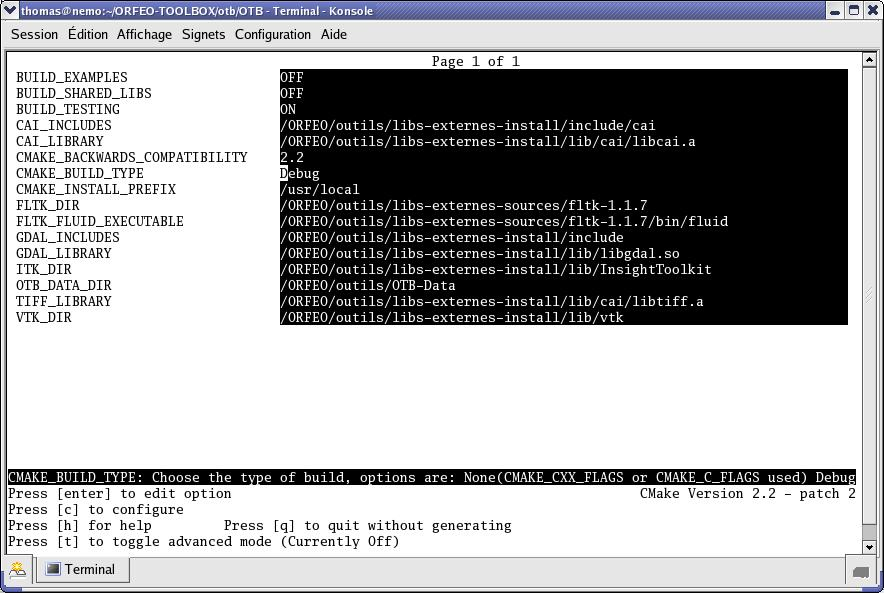
\includegraphics[width=0.8\textwidth]{ccmakeScreenShot.eps}
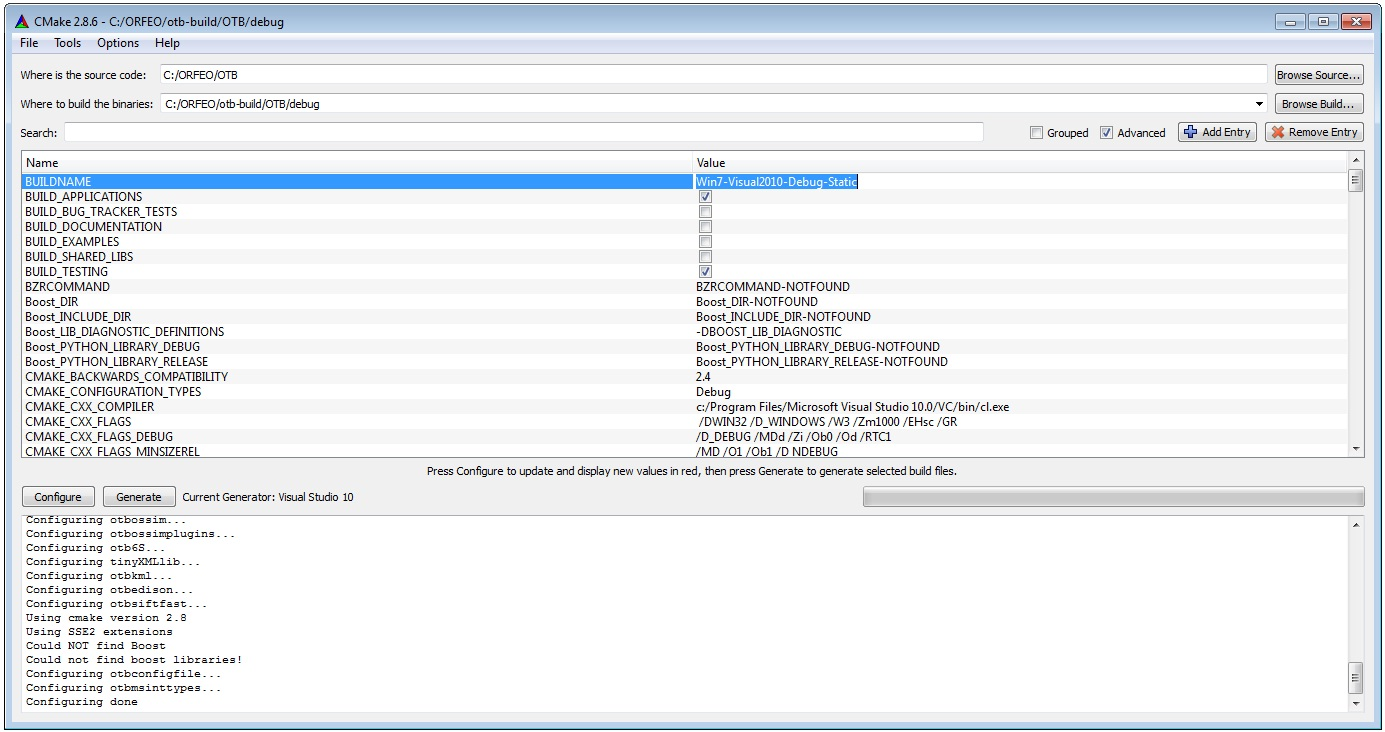
\includegraphics[width=0.8\textwidth]{CMakeSetupScreenShot.eps}
\itkcaption[Cmake user interface]{CMake interface. Top) \texttt{ccmake}, the UNIX
version based on \texttt{curses}. Bottom) \texttt{CMakeSetup}, the MS-Windows
version based on MFC.}
\label{fig:CMakeGUI}
\end{figure}

Figure \ref{fig:CMakeGUI} shows the CMake interface for UNIX and MS-Windows.
In order to speed up the build process you may want to disable the compilation
of the testing and examples. This is done with the variables
\code{BUILD\_TESTING=OFF} and \code{BUILD\_EXAMPLES=OFF}.  The examples
distributed with the toolbox are a helpful resource for learning how to use OTB
components but are not essential for the use of the toolbox itself. The testing
section includes a large number of small programs that exercise the
capabilities of OTB classes. Due to the large number of tests, enabling the
testing option will considerably increase the build time.  It is not
desirable to enable this option for a first build of the toolbox.

\code{OTB-Applications}, which contains applications incorporating GUIs and different levels
of visualization are also available. The variable \code{BUILD\_APPLICATION=ON} enables 
application building. A complete list of available applications can be found 
on \href{http://orfeo-toolbox.org/Applications/index.html}{OTB Website}

Begin running CMake by using
ccmake on Unix, and CMakeSetup on
Windows. Remember to run ccmake from the binary directory on Unix. On
Windows, specify the source and binary directories in the GUI, then begin to
set the build variables in the GUI as necessary.  Most variables should have
default values that are sensible. Each time you change a set of variables in
CMake, it is necessary to proceed to another configuration step. In the
Windows version this is done by clicking on the ``Configure'' button. In the
UNIX version this is done in an interface using the
curses library, where you can configure by hitting the ``c'' key.

When no new options appear in CMake, you can proceed to generate Makefiles or
Visual Studio projects (or appropriate build file(s) depending on your
compiler). This is done in Windows by clicking on the ``Ok'' button.  In the
UNIX version this is done by hitting the ``g'' key. After the generation
process CMake will quit silently. To initiate the build process on UNIX,
simply type \code{make} in the binary directory. Under Windows, load the
workspace named \code{OTB.dsw} (if using MSDEV) or \code{OTB.sln} (if using
the .NET compiler) from the binary directory you specified in the CMake GUI.

The build process will typically take anywhere from 15 to 30 minutes depending
on the performance of your system. If you decide to enable testing as part of
the normal build process, about 600 small test programs will be compiled. This
will verify that the basic components of OTB have been correctly built on your
system.

\subsubsection{Building ITK}

The OTB installation procedure allows you to choose between building
the OTB with an external version of ITK already present in your
system. The choice is made by using the \code{OTB\_USE\_EXTERNAL\_ITK}
CMake variable.

\section{Getting Started With OTB }
\label{sec:GettingStartedWithOTB}

The simplest way to create a new project with OTB is to create a new directory
somewhere in your disk and create two files in it. The first one is a
\code{CMakeLists.txt} file that will be used by CMake to generate a Makefile
(if you are using UNIX) or a Visual Studio workspace (if you are using
MS-Windows).  The second file is an actual C++ program that will exercise
some of the large number of classes available in OTB. The details of these files
are described in the following section.

Once both files are in your directory you can run CMake in order to configure
your project. Under UNIX, you can cd to your newly created directory
and type ``\code{ccmake .}''. Note the ``.'' in the command line for indicating
that the \code{CMakeLists.txt} file is in the current directory. The
curses interface will require you to provide the directory where OTB
was built. This is the same path that you indicated for the
\code{OTB\_BINARY\_DIR} variable at the time of configuring OTB. Under
Windows you can run CMakeSetup and provide your newly created
directory as being both the source directory and the binary directory for
your new project (i.e., an in-source build). Then CMake will require you to
provide the path to the binary directory where OTB was built. The OTB binary
directory will contain a file named \code{OTBConfig.cmake} generated during the
configuration process at the time OTB was built.  From this file, CMake will
recover all the information required to configure your new OTB project.


\subsection{Hello World !}
\label{sec:HelloWorldOTB}

\index{Hello World}

Here is the content of the two files to write in your new project. These two
files can be found in the \code{OTB/Examples/Installation} directory. The
\code{CMakeLists.txt} file contains the following lines:

\small
\begin{verbatim}
PROJECT(HelloWorld)

FIND_PACKAGE(OTB REQUIRED)
INCLUDE(${OTB_USE_FILE})

ADD_EXECUTABLE(HelloWorld HelloWorld.cxx )
TARGET_LINK_LIBRARIES(HelloWorld OTBCommon OTBIO ITKCommon ITKIO)
\end{verbatim}

\normalsize

The first line defines the name of your project as it appears in Visual
Studio (it will have no effect under UNIX). The second line loads a CMake
file with a predefined strategy for finding OTB \footnote{Similar files are
provided in CMake for other commonly used libraries, all of them named
\code{Find*.cmake}}. If the strategy for finding OTB fails, CMake will prompt
you for the directory where OTB is installed in your system. In that case you
will write this information in the \code{OTB\_DIR} variable. The line \code{
INCLUDE(\$\{USE\_OTB\_FILE\})} loads the \code{UseOTB.cmake} file to set
all the configuration information from OTB.

%The next block of lines is needed in order for CMake to know whether you
%are using the OTB's internal version of ITK or an external one. In the
%second case, CMake will try to find ITK in your system. As for OTB, if
%it fails in finding ITK, it will ask you to manually set the ITK location.

The line \code{ADD\_EXECUTABLE}
defines as its first argument the name of the executable that will be produced
as result of this project. The remaining arguments of \code{ADD\_EXECUTABLE}
are the names of the source files to be compiled and linked.  Finally, the
\code{TARGET\_LINK\_LIBRARIES} line specifies which OTB libraries will be
linked against this project.


\input HelloWorld.tex

At this point you have successfully installed and compiled OTB, and created
your first simple program. If you have difficulties, please join the
otb-users mailing list (Section~\ref{sec:JoinMailList} on page
\pageref{sec:JoinMailList}) and post questions there.
